\subsection{Image Clustering by Unit Summaries}

\begin{figure}[!htb]
\centering
  \begin{subfigure}[b]{.24\linewidth}
    \centering
    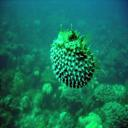
\includegraphics[width=.99\textwidth]{figures/clustering/aquarium}
    \caption{input image}\label{fig:clustering_aquarium_input}
  \end{subfigure}  \\%
  \begin{subfigure}[b]{.99\linewidth}
    \centering
    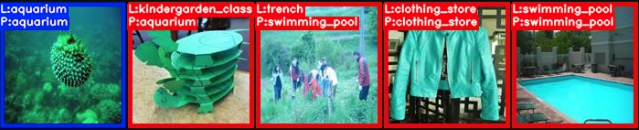
\includegraphics[width=.99\textwidth]{figures/clustering/aquarium_conv1_avg}
    \caption{conv1 cluster (avg activation unit summary)}\label{fig:clustering_aquarium_conv1}
  \end{subfigure}  \\%
  \begin{subfigure}[b]{.99\linewidth}
    \centering
    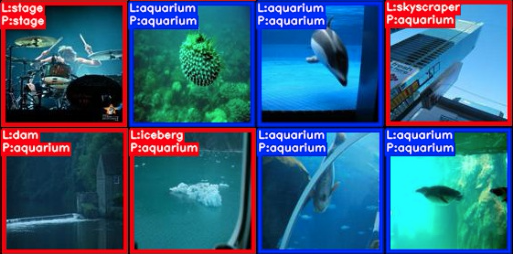
\includegraphics[width=.99\textwidth]{figures/clustering/aquarium_conv4_avg}
    \caption{conv4 cluster (avg activation unit summary)}\label{fig:clustering_aquarium_conv4}
  \end{subfigure}  \\%
  \begin{subfigure}[b]{.99\linewidth}
    \centering
    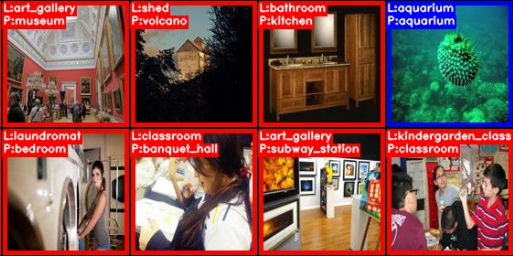
\includegraphics[width=.99\textwidth]{figures/clustering/aquarium_dhash}
    \caption{perceptual image hashing cluster (baseline, no activation information used)}\label{fig:clustering_baseline}
  \end{subfigure}%
  \caption{Figures (b) and (c) show images in the same cluster as the input ``aquarium'' image when the ``average activation'' unit summarization is used to produce each image's feature vector.  Figure (d) displays a qualitative baseline obtained by clustering input images without considering their activations, and instead using the image's perceptual hash difference as distance metric for k-means.}
  \label{fig:aquarium_clusters}
\end{figure}

In this set of experiments, we are trying to determine whether unit summaries capture enough information to suggest what granularity of semantic concept a layer learns to detect.  Recall from Figure~\ref{fig:vectorization} and Section~\ref{ss:approach_feature_vectors} that our working hypothesis is that groups of units activate in similar amounts for input images that describe semantically related scenes, or otherwise contain similar objects.  If that hypothesis is correct, then a feature vector where each dimension is a unit summary when used as basis for clustering should yield clusters with images that are visually similar with respect to concepts learned in that layer.

To validate this hypothesis, our system takes as input the validation data set and, for each image, generates a set of feature vectors that summarize activations for a given layer using one of the following aggregation functions:\\

\noindent {\bf Average activation.} In this feature vector, each activation image -- one per unit for each layer of the CNN, as shown in Figure~\ref{fig:vectorization} -- is summarized as a single value computed as average pixel intensity for all pixels in the activation image for that unit. As expected, this summary loses the location of activated pixels in the original activation image, as well as any shapes present on it, whilst keeping the relative amount of activation normalized by the activation image's size.  
%%In other words, if the CNN when fed with the image of a cat has 40\% of pixels fully activated -- pixel intensity is 1.0 -- and no other pixels activated -- pixel intensity is 0.0 -- in the 2nd unit of convolutional layer 3, then the 2nd dimension of the cat image's \texttt{conv3} feature vector is set to 0.4.

\noindent {\bf Maximum activation.} Here each activation image is summarized as the maximum pixel intensity over all pixels in the activation image, i.e., each dimension in the feature vector is set to the maximum pixel intensity observed for the corresponding activation unit in the layer.  This summary captures very little information, as it loses not only the shape and location of activations in the unit, but also the relative amount of activations.

\noindent {\bf Top 10\% maximum activations.} The value of each dimension in this feature vector is the sum of pixel intensities for the top 10\% most activated pixels in the corresponding unit's activation image.  This aggregation function sits somewhere between the average and maximum summarization steps described above, in that it loses the original shape and location of the activated pixels, while still partially retaining the relative amount of activations for a given input image.

\noindent {\bf Average activations with cutoff.} Each dimension in this feature vector starts out the same way as in the average activation summary vector.  We then set only the top 4 largest dimensions (or average activations) to 1.0 and all other dimensions to 0.  This is the most drastic of summarization strategies we have explored here, in that not only is each activation image transformed into a single value, but a second pass over the vector erases any information regarding how other units activated for the input image under consideration.

In this set of experiments, our prototype generates feature vectors for all 5 convolutional layers -- after ReLu layer -- for all 10,000 validation images in the MiniPlaces dataset.  Each feature vector has as many dimensions as the number of units in the corresponding layer: 96, 256, 384, 256 and 256 respectively for \texttt{conv1} through \texttt{conv5}. This amounts to 50,000 vectors in total (5 per image in the validation set), which are then fed into k-means clustering pipeline -- initial seed using k-means++ -- with euclidean as the distance metric.

We also built a tool that, for a given input image and summarization type, finds the clusters that the image is part of in each of the 5 convolutional layers in our AlexNet model, and visualizes them.  The tool also displays both the original class label and final prediction for each of the images in the cluster.  Finally, the cluster visualizations that the tool produces distinguish between images that are of the same class as the input image, and those that are of a different class.

Figure~\ref{fig:aquarium_clusters} shows a subset of the resulting clusters in which the input image of an aquarium falls into.  Clusters obtained from 3 different configurations of feature vectors for k-means clustering are depicted: when the feature vector is composed of the unit summaries in \texttt{conv1} in AlexNet (Figure~\ref{fig:clustering_aquarium_conv1}), the unit summaries of the \texttt{conv4} in the same network (Figure~\ref{fig:clustering_aquarium_conv4}), and a baseline cluster obtained by image similarity which disregards any information from the CNN (perceptual hash difference as distance measure).  The resulting clusters indicate that, for the input aquarium image, the units that activate on it are those which learn filters based on color transitions, since images that activate the same units in a similar way only share in common large amounts of the same shade of green.

As we go deeper on the layers of the CNN, however, images of the same class are considered similar -- likely because they activate the same units that learn to detect shapes surrounded by bodies of water.  We also get visual explanations for why certain scenes are misclassified, e.g., a skyscraper image turns up in the same cluster, likely because the large building in the image is mostly surrounded by sky which the network could have mistaken for water (both have large amounts of shades of blue).  Finally, Figure~\ref{fig:clustering_baseline} shows that the image similarity cluster obtained when no information from the CNN activations is taken into consideration fails to group images in any meaningful way.  We depict here only the resulting cluster for one of a family of perceptual hashing~\cite{phash_benchmark,imagehash} functions, but our experiments showed similar low quality clusters for all other 4 perceptual hashing functions as well.

\begin{figure}[t]
\centering
  \begin{subfigure}[b]{.24\linewidth}
    \centering
    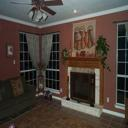
\includegraphics[width=.99\textwidth]{figures/clustering/living_room}
    \caption{input image}\label{fig:clustering_living_room_input}
  \end{subfigure}  \\%
  \begin{subfigure}[b]{.99\linewidth}
    \centering
    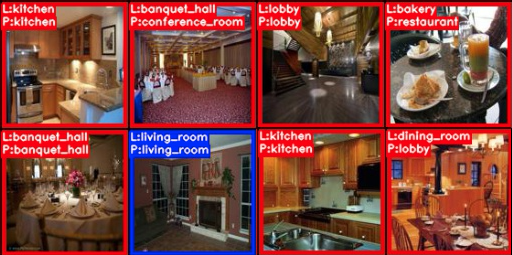
\includegraphics[width=.99\textwidth]{figures/clustering/living_room_conv4_avg}
    \caption{conv4 cluster (avg activation unit summary)}\label{fig:clustering_living_room_conv4}
  \end{subfigure}%
  \caption{Figure (b) shows images in the same cluster as the input ``living room'' scene (a) when the ``average activation'' unit summarization is used to produce each image's feature vector for k-means clustering.}
  \label{fig:living_room_cluster}
\end{figure}

Figure~\ref{fig:living_room_cluster} shows a subset of the images deemed similar to a ``living room'' scene from the validation set in MiniPlaces.  When the input image has higher concentration of complex concepts, unit summaries for deeper layers seem to activate in similar amounts for images that, despite not being from the same class as the input scene, are semantically related. More concretely, ``kitchen'', ``banquet hall'', and ``dining room'' scenes all clustered together with the input ``living room'', likely because these are all indoors images with furniture on them.  This suggests that the same units activate in similar amounts for these visual patterns on \texttt{conv4} of the AlexNet model we used for evaluation.

While it is difficult to generalize our findings without a quantitative measure of cluster ``quality'', we empirically observe from manual qualitative evaluation of randomly sampled clusters that ``average summarization'' seems to work best amongst the aggregations we consider. The rationale for why that is the case is somewhat intuitive: of the aggregation functions above, ``average summarization'' is the only one that correlates with amount of activated pixels originally present in the activation image.
